\chapter{CARP: Adaptive In-Situ Range Partitioning}

\section{Motivation: The Need for Efficient In-Situ Range Queries}

Scientific applications require efficient range queries to analyze massive simulation datasets,
enabling researchers to track phenomena like wave fronts or filter data by physical properties such
as particle energy.
However, achieving high query performance today requires expensive post-processing sorts that
re-read and re-write all data, delaying the time-to-discovery.
Existing in-situ alternatives fall short: hash-based partitioners like DeltaFS are excellent for
point queries but destroy the key ordering needed for ranges, while auxiliary indices suffer from
poor query performance due to random I/O patterns.

The fundamental challenge is to design a single-pass, streaming partitioner that can organize data
efficiently without prior knowledge of its characteristics.
Our analysis reveals that scientific key distributions are often highly skewed and evolve
significantly as a simulation progresses.
This dynamism makes any static partitioning scheme ineffective, while the high write amplification
of traditional databases makes them unsuitable for HPC's write-intensive workloads.
The goal of CARP is therefore to provide the query performance of a fully sorted index without the
associated post-processing delays or ingestion overhead.

\section{The CARP Architecture}

\begin{figure}[h]
  \centering
  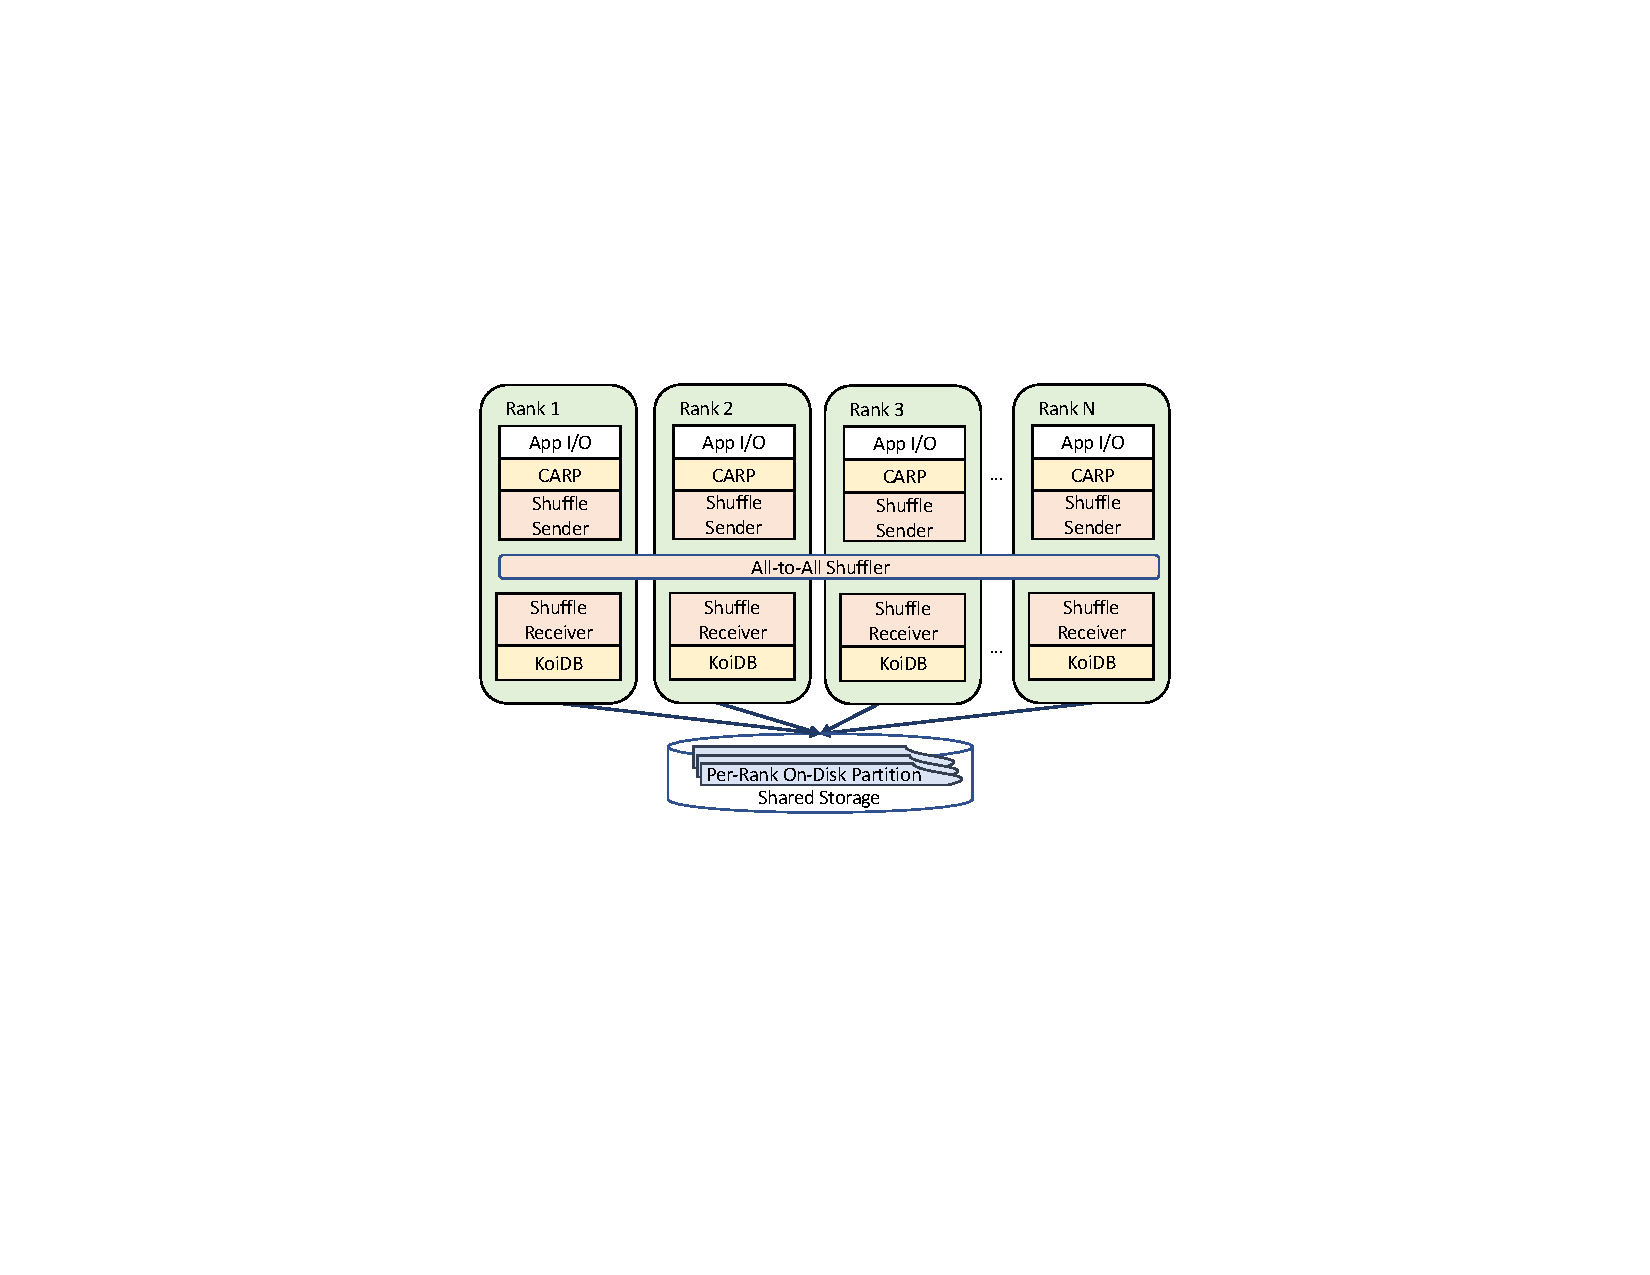
\includegraphics[
    width=0.6\textwidth,trim=8cm 7cm 8cm 6cm,clip
  ]{data/figs/carp_arch_v12mini.pdf}
  \caption{CARP architecture.}
\end{figure}

\subsection{A Streaming, In-Situ Data Reorganization Engine}

CARP is an in-situ system that intercepts application writes and reorders data on-the-fly using a
scalable all-to-all shuffle overlay.
Each application rank acts as both a sender and a receiver, shuffling data records to a destination
rank determined by the value of a user-specified key.
This process reorganizes the data stream into a range-partitioned layout before it is persisted,
creating key locality without requiring expensive on-disk reorganization.

\subsection{The Renegotiation Protocol: An Adaptive Control Loop}

The core innovation in CARP is the Renegotiation Protocol, a lightweight, distributed control loop
that allows the system to adapt to changing key distributions.
Rather than relying on static boundaries, CARP reconstructs an estimate of the global key
distribution at runtime.
Each rank maintains a local histogram of the keys it processes.
When triggered, the protocol initiates a scalable reduction, where compact summaries of these local
histograms (called pivots) are merged to form a global view.
From this reconstructed global state, a new, balanced set of partition boundaries is computed and
broadcast to all ranks.
This entire process occurs without rewriting previously stored data, enabling CARP to adapt to
distribution drift with minimal overhead.

\subsection{KoiDB: A Write-Optimized Storage Backend}

The partitioned data streams are persisted by KoiDB, CARP's reference storage backend.
KoiDB is designed for high-throughput ingestion, collecting shuffled records in memory and flushing
them to an append-only log as large, immutable blocks.
This design minimizes write amplification and aligns with the I/O patterns of parallel filesystems.

\section{Key Results}

\begin{figure}[h]
  \centering 
  \begin{subfigure}{0.48\textwidth}
    \centering
    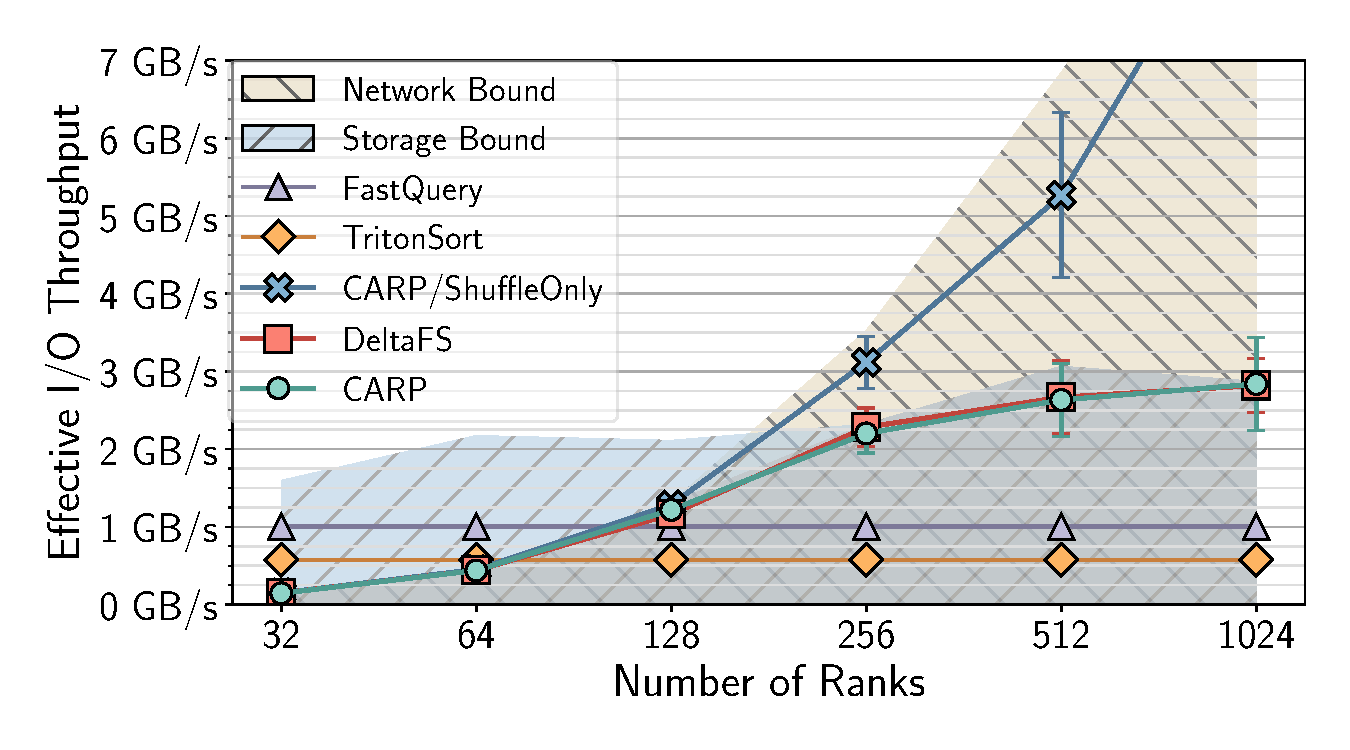
\includegraphics[
      width=\textwidth,trim=0cm 0cm 0cm 0cm,clip
      ]{data/figs/carp_runtime.v4.werr.pdf}
    \caption{Write performance.}
  \end{subfigure}
  \begin{subfigure}{0.48\textwidth}
    \centering 
    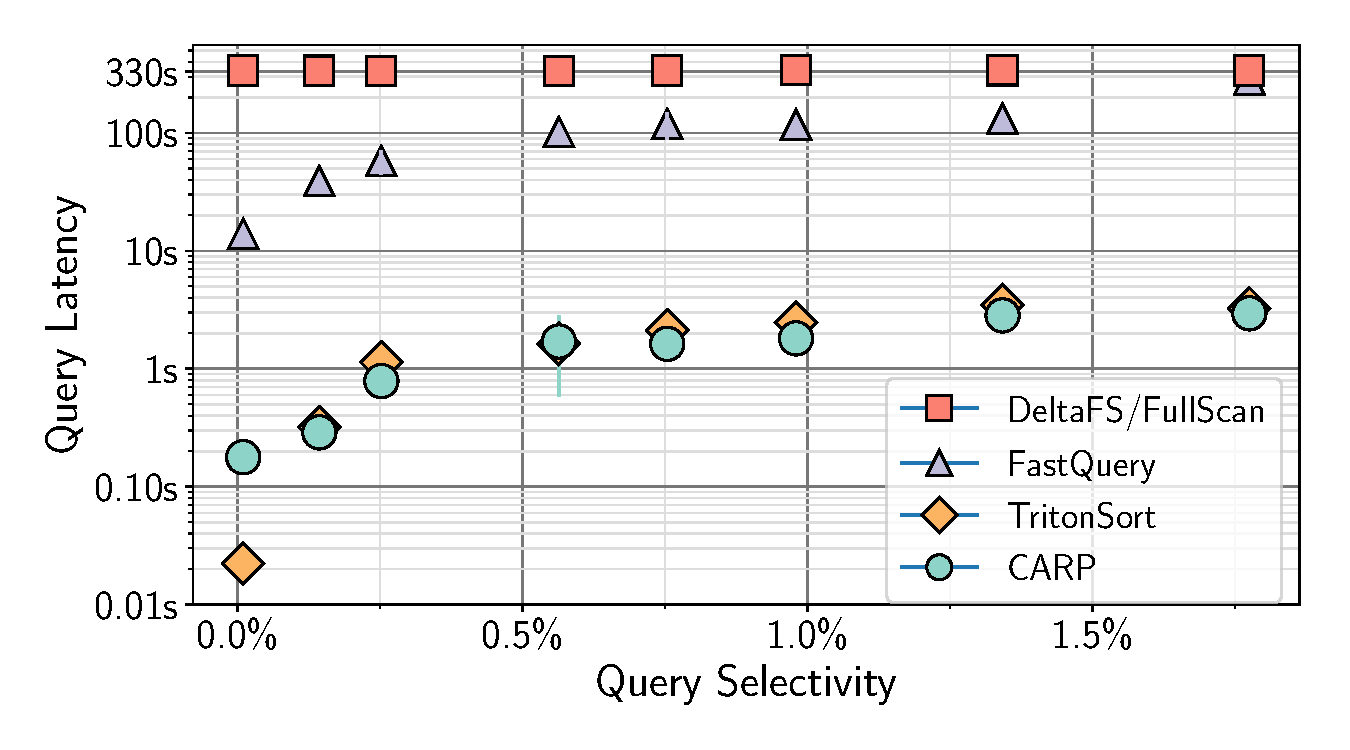
\includegraphics[
      width=\textwidth,trim=0cm 0cm 0cm 0cm,clip
      ]{data/figs/carp_qlatvssel.v6.pdf}
    \caption{Query performance.}
  \end{subfigure}
  \caption{CARP performance.}
\end{figure}

\subsection{Write Performance and End-to-End Efficiency}

CARP adds no measurable overhead to the application's I/O runtime.
By overlapping its shuffling and rebalancing work with the application's I/O phase, it fully
utilizes available network and storage bandwidth.
As a result, CARP's end-to-end workflow is up to 5x faster than approaches that require a separate,
offline post-processing sort.

\subsection{Query Performance}

For range queries, CARP's performance is comparable to that of a fully sorted, clustered index
created via an expensive offline sort.
Compared to other in-situ techniques that build auxiliary indices, CARP's range query latency is up
to 100x faster.
This is because CARP's range-partitioned layout allows queries to be served with a small number of
large, sequential reads, avoiding the performance penalty of random I/O.

\section{Lesson: Data Organization as State Reconstruction}

The success of CARP provides a key insight that informs the rest of this thesis: a complex,
distributed data organization problem can be solved by reframing it as a problem of state
reconstruction.
CARP works by building a "good enough" model of a piece of distributed state—the global key
distribution—in a streaming, online fashion.
The Renegotiation Protocol is the first example of an adaptive control loop used as a powerful tool
for data path management, a theme that will be revisited in subsequent chapters.
